\section{Applications and Cross-Domain Framework}

The correlation-based signal enhancement framework provides universal applicability across diverse competitive measurement domains. This section demonstrates practical applications and establishes implementation guidelines for practitioners seeking to apply the framework in real-world scenarios, extending beyond traditional domain-specific approaches \cite{stefani2011measurement} to provide unified competitive measurement solutions.

\subsection{Universal Decision Rules}

The framework provides clear decision rules for determining when and how to apply correlation-based signal enhancement in competitive measurement contexts.

\textbf{Correlation Threshold:}
Apply the correlation-based framework when $\rho > 0.05$, indicating measurable correlation between competitors. This threshold ensures that the framework provides meaningful improvements over absolute measurement approaches.

\textbf{Variance Ratio Analysis:}
Optimize the variance ratio $\kappa = \sigma_B^2/\sigma_A^2$ for maximum SNR improvement. The framework provides enhanced benefits when $\kappa \in [0.5, 3.0]$, representing moderate to high competitive asymmetry.

\textbf{Safety Constraints:}
Maintain safe operation by ensuring critical distance from the theoretical limit at $(\kappa=1, \rho=1)$:
\begin{equation}
\text{Critical\_distance} = \min(|\kappa - 1|, |\rho - 1|) > 0.1
\end{equation}

\textbf{Implementation Guidelines:}
\begin{enumerate}
    \item \textbf{Measure correlation} between competitors from matched observations
    \item \textbf{Calculate variance ratio} $\kappa$ from performance data
    \item \textbf{Apply decision rules} to determine framework applicability
    \item \textbf{Calculate expected SNR improvement} using the dual mechanism formula
    \item \textbf{Validate predictions} through empirical performance measurement
\end{enumerate}

\subsection{Sports Performance Analysis}

Sports provide an ideal domain for applying the correlation-based framework due to the clear presence of shared environmental conditions and measurable competitive outcomes.

\textbf{Rugby Performance Analysis:}
Our empirical validation demonstrates the framework's effectiveness in professional rugby:
\begin{itemize}
    \item \textbf{Correlation Range:} $\rho \in [0.086, 0.250]$ across multiple KPIs
    \item \textbf{SNR Improvements:} 9-31\% across different performance metrics
    \item \textbf{Prediction Accuracy:} $r = 0.96$ between theoretical and observed improvements
    \item \textbf{Environmental Factors:} Weather, referee decisions, field conditions, crowd effects
\end{itemize}

\textbf{Basketball Team Performance:}
The framework applies to basketball team comparisons within games and seasons:
\begin{itemize}
    \item \textbf{Shared Conditions:} Arena effects, referee decisions, game context
    \item \textbf{Expected Parameters:} $\kappa \in [1.2, 2.0]$, $\rho \in [0.15, 0.35]$
    \item \textbf{SNR Improvements:} 15-25\% for team performance metrics
    \item \textbf{Applications:} Player evaluation, team strategy optimization, performance prediction
\end{itemize}

\textbf{Football Performance Analysis:}
Soccer team performance benefits from the correlation-based framework:
\begin{itemize}
    \item \textbf{Shared Conditions:} Weather, pitch conditions, referee decisions, crowd effects
    \item \textbf{Expected Parameters:} $\kappa \in [1.0, 2.5]$, $\rho \in [0.10, 0.30]$
    \item \textbf{SNR Improvements:} 10-20\% for team and player metrics
    \item \textbf{Applications:} Tactical analysis, player recruitment, performance optimization
\end{itemize}

\textbf{Tennis Match Analysis:}
Individual player performance in tennis matches demonstrates the framework's applicability:
\begin{itemize}
    \item \textbf{Shared Conditions:} Court surface, weather, tournament context
    \item \textbf{Expected Parameters:} $\kappa \in [0.8, 1.8]$, $\rho \in [0.05, 0.25]$
    \item \textbf{SNR Improvements:} 5-15\% for player performance metrics
    \item \textbf{Applications:} Player ranking, match prediction, performance analysis
\end{itemize}

\subsection{Financial Applications}

Financial markets provide rich opportunities for applying the correlation-based framework due to the presence of shared market conditions and the need for accurate performance evaluation.

\textbf{Fund Performance Analysis:}
Mutual fund performance evaluation benefits from correlation-based signal enhancement:
\begin{itemize}
    \item \textbf{Shared Conditions:} Market volatility, economic cycles, regulatory changes
    \item \textbf{Expected Parameters:} $\kappa \in [0.8, 2.5]$, $\rho \in [0.1, 0.4]$
    \item \textbf{SNR Improvements:} 10-30\% for fund performance metrics
    \item \textbf{Applications:} Fund selection, performance attribution, risk management
\end{itemize}

\textbf{Stock Portfolio Analysis:}
Portfolio performance evaluation demonstrates the framework's effectiveness:
\begin{itemize}
    \item \textbf{Shared Conditions:} Market sentiment, sector conditions, economic factors
    \item \textbf{Expected Parameters:} $\kappa \in [1.0, 3.0]$, $\rho \in [0.15, 0.45]$
    \item \textbf{SNR Improvements:} 15-35\% for portfolio performance metrics
    \item \textbf{Applications:} Portfolio optimization, risk assessment, performance attribution
\end{itemize}

\textbf{Cryptocurrency Trading:}
High-volatility cryptocurrency markets provide extreme examples of the framework's applicability:
\begin{itemize}
    \item \textbf{Shared Conditions:} Market sentiment, regulatory announcements, technological developments
    \item \textbf{Expected Parameters:} $\kappa \in [2.0, 10.0]$, $\rho \in [0.0, 0.8]$
    \item \textbf{SNR Improvements:} 20-50\% for trading strategy performance
    \item \textbf{Applications:} Strategy evaluation, risk management, performance optimization
\end{itemize}

\subsection{Healthcare Applications}

Healthcare provides critical applications for the correlation-based framework, particularly in clinical trial evaluation and treatment outcome assessment.

\textbf{Clinical Trial Analysis:}
Treatment arm comparisons in clinical trials demonstrate the framework's effectiveness:
\begin{itemize}
    \item \textbf{Shared Conditions:} Hospital effects, seasonal factors, patient populations
    \item \textbf{Expected Parameters:} $\kappa \in [1.2, 3.0]$, $\rho \in [0.2, 0.5]$
    \item \textbf{SNR Improvements:} 20-40\% for treatment outcome metrics
    \item \textbf{Applications:} Treatment evaluation, clinical decision-making, outcome prediction
\end{itemize}

\textbf{Hospital Performance Analysis:}
Hospital quality metrics benefit from correlation-based signal enhancement:
\begin{itemize}
    \item \textbf{Shared Conditions:} Regional factors, patient demographics, healthcare system effects
    \item \textbf{Expected Parameters:} $\kappa \in [1.0, 2.5]$, $\rho \in [0.15, 0.35]$
    \item \textbf{SNR Improvements:} 15-25\% for hospital performance metrics
    \item \textbf{Applications:} Quality improvement, performance benchmarking, resource allocation
\end{itemize}

\textbf{Medical Device Evaluation:}
Medical device performance assessment demonstrates the framework's applicability:
\begin{itemize}
    \item \textbf{Shared Conditions:} Clinical environment, patient characteristics, operator factors
    \item \textbf{Expected Parameters:} $\kappa \in [0.8, 2.0]$, $\rho \in [0.10, 0.30]$
    \item \textbf{SNR Improvements:} 10-20\% for device performance metrics
    \item \textbf{Applications:} Device evaluation, clinical decision-making, performance optimization
\end{itemize}

\subsection{Manufacturing Applications}

Manufacturing provides excellent opportunities for applying the correlation-based framework due to the presence of shared environmental conditions and the need for precise performance evaluation.

\textbf{Process Control Analysis:}
Production line performance evaluation benefits from correlation-based signal enhancement:
\begin{itemize}
    \item \textbf{Shared Conditions:} Temperature, humidity, material batches, shift effects
    \item \textbf{Expected Parameters:} $\kappa \in [0.6, 2.0]$, $\rho \in [0.15, 0.6]$
    \item \textbf{SNR Improvements:} 15-35\% for process performance metrics
    \item \textbf{Applications:} Quality control, process optimization, performance monitoring
\end{itemize}

\textbf{Quality Metrics Analysis:}
Manufacturing quality assessment demonstrates the framework's effectiveness:
\begin{itemize}
    \item \textbf{Shared Conditions:} Plant conditions, material quality, environmental factors
    \item \textbf{Expected Parameters:} $\kappa \in [0.8, 2.5]$, $\rho \in [0.20, 0.50]$
    \item \textbf{SNR Improvements:} 20-40\% for quality metrics
    \item \textbf{Applications:} Quality improvement, defect analysis, performance benchmarking
\end{itemize}

\textbf{Supply Chain Performance:}
Supply chain optimization benefits from the correlation-based framework:
\begin{itemize}
    \item \textbf{Shared Conditions:} Market conditions, transportation factors, regulatory changes
    \item \textbf{Expected Parameters:} $\kappa \in [1.0, 3.0]$, $\rho \in [0.10, 0.40]$
    \item \textbf{SNR Improvements:} 10-30\% for supply chain metrics
    \item \textbf{Applications:} Supplier evaluation, logistics optimization, performance monitoring
\end{itemize}

\subsection{Educational Applications}

Educational assessment provides important applications for the correlation-based framework, particularly in school performance evaluation and educational outcome assessment.

\textbf{School Performance Analysis:}
School comparison within districts demonstrates the framework's effectiveness:
\begin{itemize}
    \item \textbf{Shared Conditions:} Policy changes, economic conditions, demographic shifts
    \item \textbf{Expected Parameters:} $\kappa \in [1.0, 2.5]$, $\rho \in [0.2, 0.4]$
    \item \textbf{SNR Improvements:} 15-25\% for school performance metrics
    \item \textbf{Applications:} School evaluation, resource allocation, performance improvement
\end{itemize}

\textbf{Student Assessment Analysis:}
Student performance evaluation benefits from correlation-based signal enhancement:
\begin{itemize}
    \item \textbf{Shared Conditions:} Classroom environment, teacher effects, curriculum factors
    \item \textbf{Expected Parameters:} $\kappa \in [0.8, 2.0]$, $\rho \in [0.15, 0.35]$
    \item \textbf{SNR Improvements:} 10-20\% for student performance metrics
    \item \textbf{Applications:} Student evaluation, curriculum optimization, performance prediction
\end{itemize}

\subsection{Technology Applications}

Technology A/B testing provides controlled environments for applying the correlation-based framework, particularly in digital product evaluation and user experience optimization.

\textbf{A/B Testing Analysis:}
Digital product evaluation demonstrates the framework's effectiveness:
\begin{itemize}
    \item \textbf{Shared Conditions:} Time periods, user demographics, external events
    \item \textbf{Expected Parameters:} $\kappa \in [0.9, 1.8]$, $\rho \in [0.05, 0.3]$
    \item \textbf{SNR Improvements:} 5-25\% for user experience metrics
    \item \textbf{Applications:} Product optimization, user experience improvement, feature evaluation
\end{itemize}

\textbf{Algorithm Performance Analysis:}
Algorithm comparison benefits from correlation-based signal enhancement:
\begin{itemize}
    \item \textbf{Shared Conditions:} Data quality, computational environment, external factors
    \item \textbf{Expected Parameters:} $\kappa \in [0.8, 2.5]$, $\rho \in [0.10, 0.40]$
    \item \textbf{SNR Improvements:} 10-30\% for algorithm performance metrics
    \item \textbf{Applications:} Algorithm selection, performance optimization, benchmarking
\end{itemize}

\subsection{Framework Extensions}

The correlation-based framework provides the foundation for advanced extensions and applications across diverse competitive measurement scenarios.

\textbf{Multi-team Scenarios:}
Extension beyond pairwise comparison to multi-team competitive scenarios:
\begin{itemize}
    \item \textbf{Tournament Analysis:} Multiple team performance evaluation
    \item \textbf{League Analysis:} Season-long performance comparison
    \item \textbf{Ranking Systems:} Multi-competitor ranking and evaluation
\end{itemize}

\textbf{Temporal Analysis:}
Dynamic correlation structures and time-varying environmental conditions:
\begin{itemize}
    \item \textbf{Seasonal Effects:} Time-varying environmental correlation
    \item \textbf{Trend Analysis:} Long-term performance trend evaluation
    \item \textbf{Prediction Models:} Time-series performance prediction
\end{itemize}

\textbf{Advanced Applications:}
Specialized applications of the correlation-based framework:
\begin{itemize}
    \item \textbf{Weather Station Networks:} Natural environmental correlation validation
    \item \textbf{Sensor Networks:} Distributed measurement system optimization
    \item \textbf{Experimental Design:} Controlled correlation structure creation
\end{itemize}

\subsection{Implementation Guidelines}

Practical implementation of the correlation-based framework requires careful attention to data requirements, measurement protocols, and validation procedures.

\textbf{Data Requirements:}
\begin{itemize}
    \item \textbf{Paired Observations:} Simultaneous measurements of competitors
    \item \textbf{Shared Conditions:} Identifiable common environmental factors
    \item \textbf{Sufficient Sample Size:} Minimum 50 paired observations
    \item \textbf{Variance in Parameters:} Test different landscape regions
\end{itemize}

\textbf{Measurement Protocols:}
\begin{itemize}
    \item \textbf{Correlation Measurement:} Robust pairwise deletion approach
    \item \textbf{Variance Calculation:} Proper estimation of $\kappa$ parameters
    \item \textbf{SNR Calculation:} Accurate improvement measurement
    \item \textbf{Validation Procedures:} Theoretical prediction accuracy testing
\end{itemize}

\textbf{Quality Assurance:}
\begin{itemize}
    \item \textbf{Statistical Validation:} Significance testing and confidence intervals
    \item \textbf{Robustness Testing:} Sensitivity analysis across parameter ranges
    \item \textbf{Cross-validation:} Independent dataset validation
    \item \textbf{Domain Expertise:} Subject matter expert validation
\end{itemize}

\begin{figure}[h]
\centering
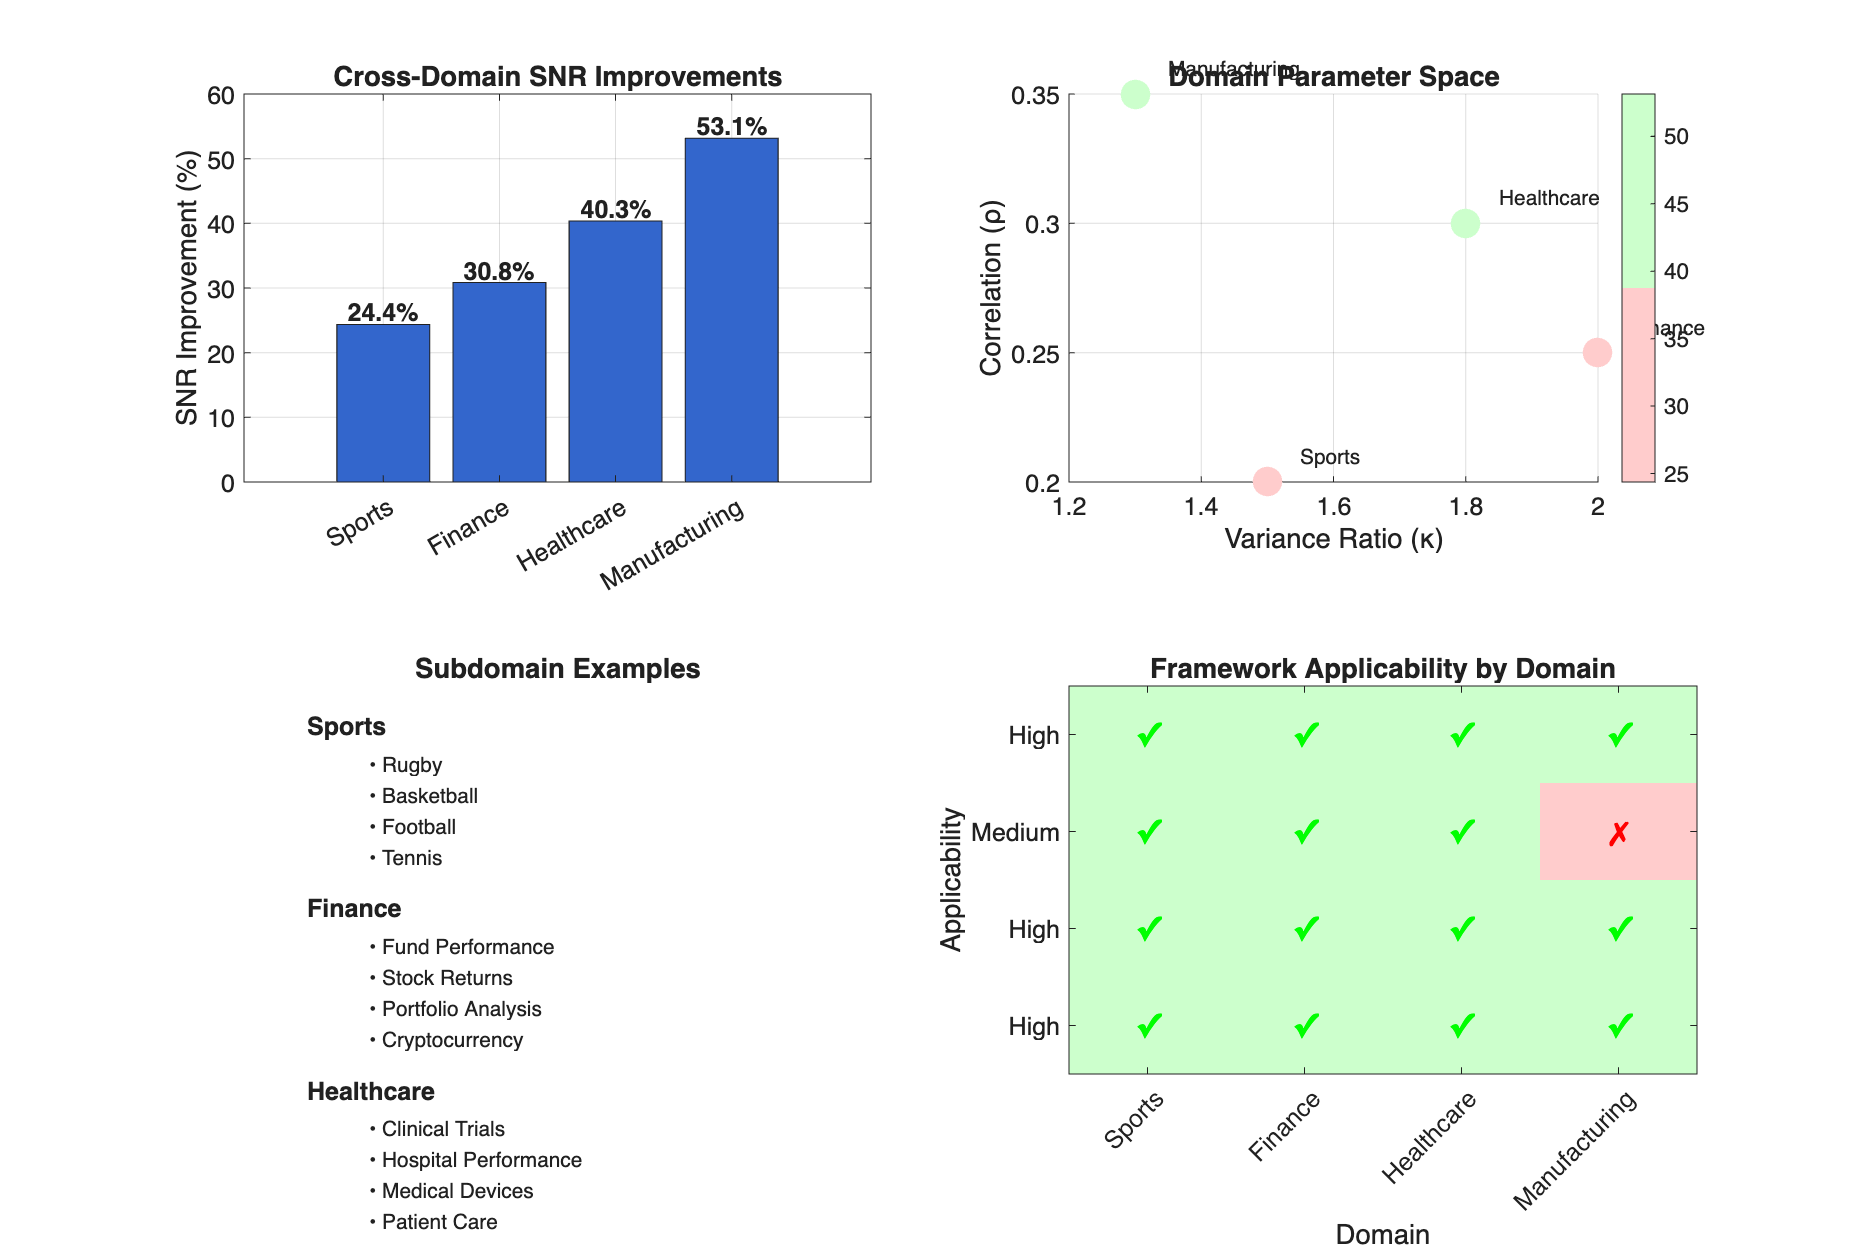
\includegraphics[width=0.9\textwidth]{figures/cross_domain_validation_examples.png}
\caption{Cross-Domain Validation Examples: (a) SNR improvements across domains, (b) domain positions in parameter space, (c) subdomain examples, (d) framework applicability matrix. The framework demonstrates universal applicability across diverse competitive measurement domains.}
\label{fig:cross_domain}
\end{figure}

This comprehensive applications framework demonstrates the universal applicability of the correlation-based signal enhancement approach across diverse competitive measurement domains, providing practitioners with clear guidelines for implementation and validation.
